\section{Package Explained}
\hspace{0.50in} LaTeX memiliki banyak fungsi secara default. Untuk mengimpor paket pada LaTeX, Anda harus menambahkan petunjuk  $ \_ $  usepackage ke pembukaan dokumen:\par

\noindent  $ \_ $ documentclass $ \{ $ article $ \} $ \par
\noindent  $ \_ $ usepackage $ \{ $ PACKAGENAME $ \} $ \par
\noindent  $ \_ $ begin $ \{ $ document $ \} $ \par

\vspace{12pt}
\hspace{0.50in} Saat menggunakan Linux atau Mac, kebanyakan paket sudah terinstal secara default dan biasanya tidak perlu menginstallnya. Jika Ubuntu menginstall texlive-full dari package manager, maka akan menyediakan semua paket yang tersedia. Bundel MiKTeX di Windows, akan mendownload paket jika dimasukkan ke dalam dokumen.\par
\hspace{0.50in} Untuk mengatur matematika, LaTeX menawarkan (antara lain) lingkungan yang disebut persamaan. Segala sesuatu di dalam lingkungan ini akan dicetak dalam mode matematika, lingkungan tata letak khusus untuk matematika. LaTeX juga menangani nomor persamaan:\par

{\fontsize{10pt}{10pt}\selectfont  $ \_ $ documentclass $ \{ $ article $ \} $ }\par

{\fontsize{10pt}{10pt}\selectfont  $ \_ $ begin $ \{ $ document $ \} $ }\par

{\fontsize{10pt}{10pt}\selectfont  $ \_ $ begin $ \{ $ equation $ \} $ }\par

{\fontsize{10pt}{10pt}\selectfont ~ f(x) = x $ \string^ $ 2}\par

{\fontsize{10pt}{10pt}\selectfont  $ \_ $ end $ \{ $ equation $ \} $ }\par

{\fontsize{10pt}{10pt}\selectfont  $ \_ $ end $ \{ $ document $ \} $ }\par
~~\noindent Hal ini akan menghasilkan output sebagai berikut: f (x) = x2 (1)\par

\vspace{12pt}
\hspace{0.50in} Penomoran otomatis adalah fitur yang berguna, namun terkadang perlu untuk menghapus perhitungan tambahan \ref{paket}:
\begin{figure}[ht]
	\centerline{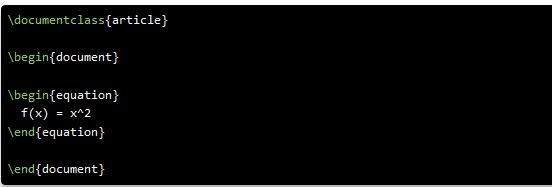
\includegraphics[width=0.70\textwidth]{gambar/paket}}
	\caption{paket}
	\label{paket}
\end{figure}

\hspace{0.50in}Hasil :
\begin{equation}
f(x) = x^2
\end{equation}

\vspace{12pt}
\hspace{0.50in} Sekarang didapat output yang sama seperti sebelumnya, hanya nomor persamaan yang dihapus: f (x) = x2.\par
\hspace{0.50in} LaTeX adalah paket makro yang banyak digunakan untuk TeX dan menyediakan banyak perintah pemformatan dokumen dasar yang diperluas oleh berbagai paket. Ini adalah pengembangan Leslie Lamport's LaTeX 2.09, dan menggantikan sistem yang lebih tua pada bulan Juni 1994. Distribusi dasar di katalogkan secara terpisah, dalam basis lateks selain dari sejumlah besar paket kontribusi dan dokumentasi pihak ketiga (di tempat lain pada arsip), distribusinya meliputi: Sekumpulan paket yang dibutuhkan, yang mana penulis LaTeX berhak untuk berasumsi akan hadir pada sistem yang menjalankan LaTeX. Seperangkat dokumentasi minimal yang merinci perbedaan dari versi 'lama' LaTeX di bidang perintah pengguna, pemilihan dan kontrol font, penulisan kelas dan paket, pengkodean font, opsi konfigurasi dan modifikasi LaTeX \par

\subsection{Daftar Kode Sumber}\par
\hspace{0.50in} Dengan menggunakan daftar paket, Anda dapat menambahkan teks yang tidak diformat seperti yang akan dilakukan dengan  $ \_ $  begin  $ \{ $ verbatim $ \} $  namun tujuan utamanya adalah memasukkan kode sumber dari bahasa pemrograman apa pun ke dalam dokumen. Jika ingin memasukkan pseudocode atau algoritma, mungkin kita dapat menemukan Algoritma dan Pseudocode berguna juga. Untuk menggunakan paket tersebut, memerlukan: 

$ \_ $  usepackage  $ \{ $ listings $ \} $

\vspace{12pt}
\hspace{0.50in}Paket daftar mendukung penyorotan semua bahasa yang paling umum dan sangat mudah disesuaikan. Jika hanya ingin menulis kode dalam dokumen, paket tersebut menyediakan lingkungan lstlisting: \par
$ \_ $  begin  $ \{ $ lstlisting $ \} $ \par

Letakkan kode anda disini  \par 
 
$ \_ $ end  $ \{ $ lstlisting $ \} $ \par
 
\vspace{12pt}
\hspace{0.50in} Kemungkinan lain, itu sangat berguna jika membuat program pada beberapa file dan masih mengeditnya, adalah dengan mengimpor kode dari sumbernya sendiri. Dengan cara ini, jika memodifikasi sumbernya, Anda hanya perlu mengkompilasi ulang kode LaTeX dan dokumen akan diperbarui. Perintahnya adalah: \par
$ \_ $  lstinputlisting  $ \{ $ source $ \_ $ filename.py $ \} $ \par

\vspace{12pt}
\hspace{0.50in} Dalam contoh ada sumber Python, tap bisa memasukkan file apapun tapi harus menulis nama file lengkap. Ini akan dianggap teks biasa dan akan disorot sesuai setting, itu berarti tidak mengenali bahasa pemrograman dengan sendirinya. Bisa menentukan bahasa sementara menyertakan file dengan perintah berikut: \par

 $ \_ $  lstinputlisting [language = Python]  $ \{ $ source $ \_ $ filename.py $ \} $ \par

\vspace{12pt}
\hspace{0.50in} Ini sangat berguna jika yakin file tersebut tidak akan berubah (setidaknya sebelum baris yang ditentukan). Menghilangkan parameter firstline atau lastline itu berarti semuanya sesuai atau dimulai dari titik ini. Ini adalah contoh dasar untuk beberapa kode Pascal:\par


\noindent  $ \_ $ documentclass $ \{ $ article $ \} $ \par


\noindent  $ \_ $ usepackage $ \{ $ listings $ \} $ ~~~~~~~~~~~~ \par


\noindent  $ \_ $ begin $ \{ $ document $ \} $ \par


\noindent  $ \_ $ lstset $ \{ $ language=Pascal $ \} $ ~~~~~~~ \par


\noindent  $ \_ $ begin $ \{ $ lstlisting $ \} $ [frame=single]~ \par


\noindent for i:=maxint to 0 do\par


\noindent begin\par


\noindent  $ \{ $  do nothing  $ \} $ \par


\noindent end;\par


\noindent Write('Case insensitive ');\par


\noindent Write('Pascal keywords.');\par


\noindent  $ \_ $ end $ \{ $ lstlisting $ \} $ \par


\noindent 
\vspace{12pt}
\noindent  $ \_ $ end $ \{ $ document $ \} $ \par


\hspace{0.50in} Memodifikasi beberapa parameter yang akan mempengaruhi bagaimana kode akan ditampilkan. Anda dapat menempatkan kode berikut di manapun dalam dokumen (tidak masalah apakah sebelum atau sesudah  $ \_ $  begin  $ \{ $ document $ \} $ ). \par
\hspace{0.50in} Paket ini memungkinkan menentukan gaya, yaitu profil yang menentukan satu set pengaturan. \par
 $ \_ $ lstdefinestyle $ \{ $ customc $ \} $  $ \{ $ \par

{\fontsize{10pt}{10pt}\selectfont ~ belowcaptionskip=1 $ \_ $ baselineskip,}\par

{\fontsize{10pt}{10pt}\selectfont ~ breaklines=true,}\par

{\fontsize{10pt}{10pt}\selectfont ~ frame=L,}\par

{\fontsize{10pt}{10pt}\selectfont ~ xleftmargin= $ \_ $ parindent,}\par

{\fontsize{10pt}{10pt}\selectfont ~ language=C,}\par

{\fontsize{10pt}{10pt}\selectfont ~ showstringspaces=false,}\par

{\fontsize{10pt}{10pt}\selectfont ~ basicstyle= $ \_ $ footnotesize $ \_ $ ttfamily,}\par

{\fontsize{10pt}{10pt}\selectfont ~ keywordstyle= $ \_ $ bfseries $ \_ $ color $ \{ $ green!40!black $ \} $ ,}\par

{\fontsize{10pt}{10pt}\selectfont ~ commentstyle= $ \_ $ itshape $ \_ $ color $ \{ $ purple!40!black $ \} $ ,}\par

{\fontsize{10pt}{10pt}\selectfont ~ identifierstyle= $ \_ $ color $ \{ $ blue $ \} $ ,}\par

{\fontsize{10pt}{10pt}\selectfont ~ stringstyle= $ \_ $ color $ \{ $ orange $ \} $ ,}\par

{\fontsize{10pt}{10pt}\selectfont  $ \} $ }\par

{\fontsize{10pt}{10pt}\selectfont  $ \_ $ lstdefinestyle $ \{ $ customasm $ \} $  $ \{ $ }\par

{\fontsize{10pt}{10pt}\selectfont ~ belowcaptionskip=1 $ \_ $ baselineskip,}\par

{\fontsize{10pt}{10pt}\selectfont ~ frame=L,}\par

{\fontsize{10pt}{10pt}\selectfont ~ xleftmargin= $ \_ $ parindent,}\par

{\fontsize{10pt}{10pt}\selectfont ~ language=[x86masm]Assembler,}\par

{\fontsize{10pt}{10pt}\selectfont ~ basicstyle= $ \_ $ footnotesize $ \_ $ ttfamily,}\par

{\fontsize{10pt}{10pt}\selectfont ~ commentstyle= $ \_ $ itshape $ \_ $ color $ \{ $ purple!40!black $ \} $ ,}\par

{\fontsize{10pt}{10pt}\selectfont  $ \} $ }\par

{\fontsize{10pt}{10pt}\selectfont  $ \_ $ lstset $ \{ $ escapechar=@,style=customc $ \} $ }\par

\vspace{12pt}
\hspace{0.50in} Dalam contoh hanya menetapkan dua pilihan secara global yaitu gaya default dan karakter escape. Pemakaian:\par

{\fontsize{10pt}{10pt}\selectfont  $ \_ $ begin $ \{ $ lstlisting $ \} $ }\par

{\fontsize{10pt}{10pt}\selectfont  $\#$ include <stdio.h>}\par

{\fontsize{10pt}{10pt}\selectfont  $\#$ define N 10}\par

{\fontsize{10pt}{10pt}\selectfont /* Block}\par

{\fontsize{10pt}{10pt}\selectfont  * comment */}\par

{\fontsize{10pt}{10pt}\selectfont int main()}\par

{\fontsize{10pt}{10pt}\selectfont  $ \{ $ }\par

{\fontsize{10pt}{10pt}\selectfont ~~~ int i;}\par

{\fontsize{10pt}{10pt}\selectfont ~~~ // Line comment.}\par

{\fontsize{10pt}{10pt}\selectfont ~~~ puts("Hello world!");}\par

{\fontsize{10pt}{10pt}\selectfont ~~~ }\par

{\fontsize{10pt}{10pt}\selectfont ~~~ for (i = 0; i < N; i++)}\par

{\fontsize{10pt}{10pt}\selectfont ~~~  $ \{ $ }\par

{\fontsize{10pt}{10pt}\selectfont ~~~~~~~ puts("LaTeX is also great for programmers!");}\par

{\fontsize{10pt}{10pt}\selectfont ~~~  $ \} $ }\par

{\fontsize{10pt}{10pt}\selectfont ~~~ return 0;}\par

{\fontsize{10pt}{10pt}\selectfont  $ \} $ }\par

{\fontsize{10pt}{10pt}\selectfont  $ \_ $ end $ \{ $ lstlisting $ \} $ }\par

{\fontsize{10pt}{10pt}\selectfont  $ \_ $ lstinputlisting[caption=Scheduler, style=customc] $ \{ $ hello.c $ \} $ }\par

\vspace{12pt}
\hspace{0.50in} Jika memiliki banyak file sumber yang ingin disertakan, mungkin mendapati diri melakukan hal yang sama berulang-ulang. 

$ \_ $  newcommand  $ \{ $  $ \_ $  includecode $ \} $  [2] [c]  $ \{ $  $ \_ $  lstinputlisting [caption =  $\#$  2, escapechar =, style = custom  $\#$  1]  $ \{ $  $\#$  2 $ \} $  <! ----> $ \} $  $\%$  ... 

$ \_ $  includecode  $ \{ $ sched.c $ \} $ 

$ \_ $  includecode [asm]  $ \{ $ sched.s $ \} $ 

$\%$  ... 

$ \_ $  lstlistoflistings

\vspace{12pt}
\hspace{0.50in} Membuat satu perintah untuk memudahkan penyertaan kode sumber. Semua daftar akan memiliki nama sebagai caption dan Anda tidak perlu menuliskan nama file dua kali kepada makro. Akhirnya semua daftar dengan perintah ini dari daftar paket. Dapat memiliki caption mewah (atau judul) untuk cantuman menggunakan paket teks. Berikut adalah contoh untuk daftar:\par

{\fontsize{10pt}{10pt}\selectfont  $ \_ $ usepackage $ \{ $ caption $ \} $ }\par

{\fontsize{10pt}{10pt}\selectfont  $ \_ $ usepackage $ \{ $ listings $ \} $ }\par

{\fontsize{10pt}{10pt}\selectfont  $ \_ $ DeclareCaptionFont $ \{ $ white $ \} $  $ \{ $   $ \_ $ color $ \{ $ white $ \} $   $ \} $ }\par

{\fontsize{10pt}{10pt}\selectfont  $ \_ $ DeclareCaptionFormat $ \{ $ listing $ \} $  $ \{ $ }\par

{\fontsize{10pt}{10pt}\selectfont ~  $ \_ $ colorbox[cmyk] $ \{ $ 0.43, 0.35, 0.35,0.01  $ \} $  $ \{ $ }\par

{\fontsize{10pt}{10pt}\selectfont ~~~  $ \_ $ parbox $ \{ $  $ \_ $ textwidth $ \} $  $ \{ $  $ \_ $ hspace $ \{ $ 15pt $ \} $  $\#$ 1 $\#$ 2 $\#$ 3 $ \} $ }\par

{\fontsize{10pt}{10pt}\selectfont ~  $ \} $ }\par

{\fontsize{10pt}{10pt}\selectfont  $ \} $ }\par

{\fontsize{10pt}{10pt}\selectfont  $ \_ $ captionsetup[lstlisting] $ \{ $  format=listing, labelfont=white, textfont=white, singlelinecheck=false, margin=0pt, font= $ \{ $ bf,footnotesize $ \} $   $ \} $ }\par

{\fontsize{10pt}{10pt}\selectfont  $ \_ $ lstinputlisting[caption=My caption] $ \{ $ sourcefile.lang $ \} $ }\par

\vspace{12pt}
\hspace{0.50in} Dicetak adalah alternatif untuk daftar yang telah menjadi populer. Menggunakan Python eksternal perpustakaan Pygments untuk menyoroti kode, yang pada November 2014 menawarkan lebih dari 300 bahasa dan format teks yang didukung. Karena paket bergantung pada kode Python eksternal, penyiapan memerlukan beberapa langkah lebih banyak daripada paket LaTeX biasa, jadi mohon lihat repo GitHub dan manualnya.\par

\subsection {Memasang Paket Ekstra}\par
\hspace{0.50in} Add-on fitur untuk LaTeX dikenal sebagai paket. Puluhan ini sudah terinstal dengan LaTeX dan dapat segera digunakan dalam dokumen. Harus disimpan di subdirektori texmf / tex / lateks dinamai setiap paket. Nama direktori "texmf" adalah singkatan dari "TEX and METAFONT". Untuk mengetahui paket apa saja yang tersedia dan apa yang dilakukan, harus menggunakan halaman pencarian CTAN yang mencakup tautan ke katalog komprehensif Graham Williams.\par

\hspace{0.50in} Paket adalah file atau kumpulan file yang berisi perintah dan pemrograman LaTeX tambahan yang menambahkan fitur styling baru atau memodifikasi yang sudah ada. Ada dua jenis file utama: file kelas dengan ekstensi .cls, dan file gaya dengan ekstensi .sty. Ketika mencoba untuk mengeset dokumen yang memerlukan paket yang tidak diinstal pada sistem, LaTeX akan memperingatkan dengan pesan kesalahan bahwa itu hilang. Mendownload update ke paket yang sudah dimiliki. Tidak ada batasan jumlah paket yang bisadi instal di komputer. Namun ada batasan yang dapat dikonfigurasi untuk nomor yang dapat digunakan di dalam dokumen LaTeX mana pun pada saat yang bersamaan, walaupun tergantung seberapa besar setiap paketnya. Dalam prakteknya tidak ada masalah dalam memiliki bahkan beberapa lusin paket yang aktif.\par

\hspace{0.50in} Kebanyakan instalasi LaTeX hadir dengan serangkaian paket gaya pra-instal yang besar, sehingga dapat menggunakan manajer paket distribusi TeX atau yang ada di sistem untuk mengelolanya. Tempat utama untuk mencari paket gaya di Internet adalah CTAN. Setelah mengidentifikasi paket yang dibutuhkan yang tidak ada dalam distribusi, gunakan indeks pada server CTAN untuk menemukan paket yang dibutuhkan dan direktori tempat downloadnya. Cara memasang paket extra :\par
\begin{enumerate}
\item Instalasi otomatis\par

\hspace{0.50in} Jika pada sistem operasi dengan manajer paket atau pohon portage, dapat sering menemukan paket di repositori. \par

\hspace{0.50in} Dengan MikTeX ada manajer paket yang memungkinkan memilih paket yang diinginkan secara individu. Sebagai fitur yang mudah digunakan, pada kompilasi sebuah file yang membutuhkan paket yang tidak terinstal, MikTeX secara otomatis akan meminta untuk menginstal yang hilang.

\hspace{0.50in} Dengan TeX Live, biasanya ada distribusi yang dikemas dalam beberapa paket besar. Untuk menginstal sesuatu yang berhubungan dengan internasionalisasi, memungkin harus menginstal paket seperti texlive-lang. Dengan TeX Live terpasang secara manual, gunakan tlmgr untuk mengelola paket secara terpisah :
\begin{verbatim}
tlmgr install <package1> <package2> ... \par

tlmgr hapus <package1> <package2> ...\par
\end{verbatim}

\item Instalasi manual\par
\hspace{0.50in} Yang perlu dicari biasanya ada dua file, yang diakhiri dengan .dtx dan .ins. Yang pertama adalah file DOCTeX yaitu menggabungkan program paket dan dokumentasinya dalam satu file. Yang kedua adalah rutin instalasi (jauh lebih kecil). Harus mendownload kedua file tersebut. Jika kedua file itu tidak ada, itu berarti satu dari dua hal:     Paket itu adalah bagian dari paket yang jauh lebih besar yang seharusnya tidak diperbarui kecuali mengubah versi LaTeX dari LaTeX atau paket itu yang lebih tua atau sederhana yang ditulis oleh seorang penulis yang tidak menggunakan file .dtx.Download file paket ke direktori sementara. Akan ada readme.txt dengan deskripsi singkat tentang paketnya.  Ada lima langkah untuk menginstal paket LaTeX. Diantaranya :

\vspace{50pt}
\noindent a. Ekstrak file\par
\hspace{0.50in}Jalankan LaTeX pada file .ins. Buka file di editor dan mengolahnya seolah-olah itu adalah dokumen LaTeX atau ketik lateks diikuti oleh nama file .ins di jendela perintah di direktori. Ini akan mengekstrak semua file yang dibutuhkan dari berkas .dtx. Catat atau cetak nama file yang dibuat jika ada banyak file tersebut (baca file log jika ingin melihat namanya lagi). \par

\vspace{10pt}
\noindent b. Buat dokumentasi \par
\hspace{0.50in} Jalankan LaTeX pada file .dtx. Membuat file dokumentasi yang menjelaskan paketnya dan cara menggunakannya. Jika lebih suka membuat PDF maka jalankan pdfLaTeX sebagai gantinya. Jika membuat .idx juga, itu berarti dokumen itu berisi indeks juga. Jika indeks dibuat dengan benar, ikuti langkah-langkah di bagian pengindeksan. Jalankan perintah berikut sebagai gantinya: \par

makeindex -s gglo.ist -o name.gls name.glo \par

\vspace{10pt}
\noindent c. Instal file\par
\hspace{0.50in}Sementara dokumentasi sedang mencetak, memindahkan atau menyalin file paket dari direktori sementara ke tempat yang tepat di pohon direktori instalasi TeX lokal\par

\hspace{0.50in} Paket yang dipasang dengan tangan harus selalu ditempatkan di pohon direktori lokal, bukan di pohon direktori yang berisi semua paket pra-instal. Hal ini dilakukan untuk mencegah paket baru secara tidak sengaja menimpa file dalam direktori utama TeX dan meghindari file yang baru diinstal yang ditimpa saat memperbarui versi TeX berikutnya.\par

\hspace{0.50in}Untuk TDS (Struktur Direktori TeX) - sistem yang sesuai, pohon direktori instalasi lokal adalah folder dan subfoldernya. Folder terluar mungkin bisa disebut texmf-local / or texmf /. Lokasinya tergantung pada sistem :        

MacTeX: Pengguna / nama pengguna / Perpustakaan / texmf/. \par     
Sistem tipe Unix: Biasanya  $ \sim $  / texmf /. \par       
MikTeX: Pohon direktori lokal \par

\vspace{8pt}
\hspace{0.50in}Jika instalasi TeX sudah tua atau tidak sesuai dengan Struktur Direktori TeX (TDS). Untuk sistem yang sesuai dengan TDS, tempat yang tepat untuk berkas LaTeX .sty adalah subdirektori texmf / tex / lateks yang sesuai.\par

\vspace{8pt}
\noindent d. Update index  \par
\hspace{0.50in} Jalankan program TeX indexer untuk mengupdate database paket. Program ini hadir dengan setiap versi modern TeX dan memiliki berbagai nama tergantung pada distribusi LaTeX yang digunakan. Sebagai berikut :\par

teTeX, TeX Live, fpTeX: texhash \par
web2c: mktexlsr \par
MacTeX: MacTeX muncul untuk melakukan ini \par
MikTeX: initexmf --update-fndb (atau gunakan GUI)
MiKTeX 2.7 atau yang lebih baru, diinstal pada Windows XP melalui Windows 7 \par

\begin{table}[ht]
	\caption{Instalasi Paket}
	\centering
	\begin{tabular}{cccc}
		\hline
		Type&Direktori&Penjelasan&\\
		\hline
		.afm&fonts/afm/foundry/typeface&Jenis huruf Adobe Font Metrics untuk font Tipe 1&\\
		.bib&bibtex/bib/bibliography&BibTeX bibliografi&\\
		.bst&bibtex/bst/packagename& gaya BibTeX&\\
		.cls&tex/latex/base& file kelas dokumen&\\
		.dvi&doc&Dokumentasi paket doc&\\
		.enc&fonts/enc&encoding font&\\
		.fd&tex/latex/mfnfss&Font Definisi file untuk font METAFONT&\\
		.fd&tex/latex/psnfss& Font Definisi file untuk font PostScript Type 1&\\
		.map&fonts/map&Font pemetaan file&\\
		.mf&fonts/source/public/typeface&METAFONT outline&\\
		.pdf&doc&documentation&\\
		.pfb&fonts/type1/foundry/typeface&huruf PostScript Type 1&\\
		.sty&tex/latex/packagename&File gaya: isi paket normal&\\
		.tex&doc&TeX sumber untuk dokumentasi paket&\\
		.tex&tex/plain/packagename&file makro Plain TeX&\\
		.tfm&fonts/tfm/foundry/typeface&TeX Font Metrics untuk font METAFONT dan Type 1&\\
		.ttf&fonts/truetype/foundry/typeface&TrueType font&\\
		.vf&fonts/vf/foundry/typeface&font virtual TeX&\\
	    others&tex/latex/packagename&jenis file lainnya kecuali diinstruksikan sebaliknya&\\		
		\hline
	\end{tabular}
\end{table}

\vspace{12pt} \par 
\noindent e. Memperbarui peta \par
\hspace{0.50in} Jika paket menginstal font TrueType atau Type 1, perlu memperbarui file pemetaan font dan memperbarui indeks. Pengarang paket harus menyertakan file .map untuk font. Program update peta biasanya beberapa varian pada updmap, tergantung pada distribusi: 
\begin{itemize}
\item TeX Live dan MacTeX: updmap --enable Map = mapfile.map (jika Anda menginstal file di pohon pribadi) atau peta updmap-sys --enable = mapfile.map (jika Anda menginstal file dalam direktori sistem) \par

\item MikTeX: Jalankan initexmf --edit-config-file updmap, tambahkan baris "Map mapfile.map ke file yang terbuka, lalu jalankan initexmf --mkmaps. \par
\end{itemize}

\vspace{12pt}
\hspace{0.50in} Alasan proses ini belum otomatis banyak adalah masih ada ribuan instalasi yang tidak sesuai dengan TDS, seperti sistem Unix bersama lama dan beberapa sistem Microsoft Windows, jadi tidak ada cara untuk program instalasi menebak dimana letakkan arsipnya. Ada juga sistem di mana pemilik, pengguna, atau pemasang telah memilih untuk tidak mengikuti struktur direktori TDS yang disarankan, atau tidak dapat melakukannya karena alasan politis atau keamanan (seperti sistem bersama yang pengguna tidak dapat menulis ke direktori yang dilindungi). Alasan untuk memiliki direktori texmf-local (disebut texmf.local pada beberapa sistem) adalah menyediakan tempat untuk modifikasi lokal atau pembaruan pribadi, terutama jika pengguna sistem bersama atau dikelola (Unix, Linux, VMS, Windows NT / 2000 / XP, dll.) Di mana pengguna mungkin tidak memiliki akses tulis ke pohon direktori instalasi TeX utama. Instalasi harus dikonfigurasi untuk mencari di direktori ini terlebih dahulu, semua instalasi TeX modern harus melakukan ini jika tidak bisa mengedit texmf / web2c / texmf.cnf sendiri.\par

\vspace{12pt}
\item Memeriksa status paket\par
\hspace{0.50in} Cara universal untuk memeriksa apakah file yang tersedia untuk kompiler TeX adalah tool command-line kpsewhich :\par 
$\$$  kpsewhich tikz \par
/usr/local/texlive/2012/texmf-dist/tex/plain/pgf/frontendlayer/tikz.tex \par
\hspace{0.50in} kpsewhich sebenarnya akan mencari file saja, bukan untuk paket. Ini mengembalikan path ke file. Untuk detail lebih lanjut tentang paket tertentu gunakan tool baris perintah tlmgr (TeX Live): \par
tlmgr info (paket)\par
\hspace{0.50in} Alat tlmgr memiliki lebih banyak pilihan. Untuk berkonsultasi dengan dokumentasi: \par
tlmgr bantuan\par

\vspace{12pt}
\item Dokumentasi paket \par
\hspace{0.50in} Untuk mengetahui apa perintah yang diberikan paket (dan bagaimana cara menggunakannya), perlu membaca dokumentasi. Di subdirektori texmf / doc dari instalasi harus ada direktori yang berisi file .dvi, satu untuk setiap paket yang diinstal. Lokasi ini khusus untuk distribusi, namun biasanya ditemukan:\par

\begin{table}[ht]
	\caption{Dokumentasi Paket}
	\centering
	\begin{tabular}{cccc}
		\hline
		Jalur&Distribusi\\
		\hline
		MacTeX &/Library / TeX / Dokumentasi / texmf-doc / lateks&\\
		MiKTeX&MIKTEXDIR\ doc \ latex&\\
		TeX Live&TEXMFDIST / doc / lateks&\\
		\hline
	\end{tabular}
\end{table}

\hspace{0.50in} Umumnya sebagian besar paket ada di subdirektori lateks, walaupun paket lainnya (seperti paket BibTeX dan font) terdapat di subdirektori lain di doc. Direktori dokumentasi memiliki nama paket yang sama, umumnya memiliki satu atau lebih dokumen yang relevan dalam berbagai format (dvi, txt, pdf, dll.). Dokumen umumnya memiliki nama yang sama dengan paketnya, namun ada pengecualian (misalnya, dokumentasi untuk amsmath ditemukan di latex / amsmath / amsdoc.dvi). Jika prosedur instalasi belum menginstal dokumentasi, file DVI semuanya dapat didownload dari CTAN. Sebelum menggunakan paket, harus membaca dokumentasi dengan seksama, terutama subseksi yang biasa disebut User Interface, yang menjelaskan perintah yang tersedia dalam paket. Membuka dokumentasi paket terinstal dengan perintah texdoc: \par
texdoc (package-name)\par
\end{enumerate}

\subsection {Referensi Paket}\par
\hspace{0.50in} Ini adalah daftar paket berguna yang tidak lengkap dapat digunakan untuk berbagai jenis dokumen yang berbeda. Setiap paket memiliki deskripsi singkat bila tersedia ada tautan ke bagian yang menjelaskan paket tersebut secara rinci. Semua (kecuali dinyatakan) harus disertakan dalam distribusi LaTeX sebagai package $ \_ $ name.sty. 

\begin{table}[ht]
	\caption{Referensi Paket}
	\centering
	\begin{tabular}{cccc}
		\hline
		amsmath&Dokumentasi yang lengkap harus ada dalam distribusi LaTeX file tersebut disebut amsdoc,dan bisa dvi atau pdf&\\
		amssymb&Ini menambahkan simbol baru untuk digunakan dalam mode matematika.&\\
		amsthm&Ini mengenalkan lingkungan bukti dan perintah theoremstyle. Untuk informasi lebih lanjut, lihat bagian Theorems&\\
		array&Ini memperluas kemungkinan LaTeX untuk menangani tabel, memperbaiki beberapa bug dan menambahkan fitur baru&\\
		babel&Ini menyediakan internasionalisasi LaTeX. &\\
		biblatex&Penanganan bibliografi tingkat lanjut&\\
		bm&Memungkinkan penggunaan huruf tebal huruf tebal dalam mode matematika menggunakan perintah \ bm {...}. Ini menggantikan paket amsbsy.&\\
		booktabs&Panduan diberikan untuk mengetahui apa yang ada dalam dokumentasi paket&\\
		boxedminipage&Ini mengenalkan lingkungan boxedminipage, yang bekerja persis seperti minipage namun menambahkan bingkai di sekitarnya&\\
		caption&Memungkinkan penyesuaian tampilan dan penempatan teks untuk angka, tabel, dll.&\\
		cancel&Menyediakan perintah untuk menunjukkan ekspresi matematis. Sintaksnya\ cancel {x} atau \ cancelto {0} {x}&\\
		chemmacros&Bagian dari kumpulan untuk mengatur kimia dengan mudah dan konsisten&\\
		changepage&Semua argumen bisa menjadi bilangan positif dan negatif, akan ditambahkan (menjaga tanda) ke variabel relatif&\\
		dcolumn&Paket tersebut mendefinisikan format kolom "D" baru di lingkungan tabular untuk menyelaraskan angka pada kolom pada titik desimal&\\
		enumitem&Menambahkan dukungan untuk daftar bersarang yang sewenang-wenang (berguna untuk garis besar)&\\
		epstopdf&Menyediakan dan pilihan untuk mengkonversi gambar EPS ke PDF dan memasukkannya ke \ includegraphics {}&\\
		esint&Menambahkan simbol integral tambahan, untuk integral di atas kotak, integral searah jarum jam di atas set, dll&\\
		eucal&Simbol matematika lainnya.&\\
		fancyhdr&Untuk mengubah header dan footer halaman manapun dari dokumen. Hal ini dijelaskan di bagian Tata Letak Halaman&\\
		float&Menghasilkan antarmuka untuk menentukan objek terapung seperti gambar dan tabel, memperkenalkan tipe benda mengambang baru &\\
		fontenc&Untuk memilih pengkodean font dari teks output&\\
		gensymb&Menyediakan perintah generik \ derajat, \ celsius, \ perthousand, \ mikro dan \ ohm yang bekerja baik dalam mode teks dan matematika&\\
		geometry&Untuk kemudahan pengelolaan margin dokumen dan ukuran halaman dokumen&\\
		glossaries&Untuk pembuatan glosarium dan daftar akronim&\\
		graphicx&Memungkinkan untuk memasukkan file grafis dalam dokumen&\\
		grffile&Memperbaiki pemrosesan nama file dari paket grafis / grafis untuk mendukung berbagai jenis nama file (spasi, beberapa titik, dll)&\\
		hyperref&Ini memberi LaTeX kemungkinan untuk mengelola tautan dalam dokumen atau URL apa pun saat mengkompilasi dalam PDF&\\
		indentfirst&Setelah dimuat, awal setiap bab / bagian diindentasikan oleh indentasi paragraf yang biasa&\\
		inputenc&Untuk memilih pengkodean teks masukan. Periksa di bagian Karakter Khusus&\\
		latexsym&Simbol matematika lainnya&\\
			mathrsfs&Simbol matematika lainnya&\\
		mathtools&Penerus amsmath, beberapa fungsi tambahan, beberapa bug tetap&\\
	\end{tabular}
\end{table}
\begin{table}[ht]
	\centering
	\begin{tabular}{cccc}
		listings&Untuk memasukkan kode pemrograman ke dalam dokumen&\\
		mathptmx&Menetapkan font default dari keseluruhan dokumen (termasuk rumus matematika) ke Times New Roman, yang merupakan font yang lebih familiar, dan berguna dalam menghemat ruang saat bertarung melawan batas halaman&\\
		mhchem&Ini memberikan perbaikan pada ekstensi tipografi default LaTeX, peningkatan pada area seperti penonjolan karakter dan perluasan font, jarak antar kata dan kerning tambahan, dan jarak huruf yang dapat dihilangkan&\\
		multicol&Menyediakan lingkungan multicols yang mengarsipkan teks menjadi beberapa kolom&\\
		natbib&Memberikan pilihan dan gaya kutipan tambahan&\\
		pdfpages&Paket ini menyederhanakan penyisipan dokumen PDF multi-halaman eksternal atau PS&\\
		rotating&Ini memungkinkan memutar objek apa pun. Hal ini sangat berguna untuk memutar meja&\\
		setspace&Memungkinkan mengubah spasi baris, mis. memberikan perintah \ doublespacing untuk membuat dokumen spasi ganda&\\
		showkeys&Jika ingin referensi gambar atau formula,  memberinya nama menggunakan \ label {...} dan dapat mengingatnya dengan menggunakan \ ref {...}&\\
		showidx&Ini sangat berguna untuk mengoreksi dokumen dan memverifikasi indeks&\\
		subfiles&Dokumen akar dan anak dapat disusun bersamaan tanpa membuat perubahan pada dokumen anak&\\
		subcaption&Hal ini memungkinkan untuk mendefinisikan beberapa pelampung (gambar, tabel) dalam satu lingkungan yang memberi caption dan label individual dalam bentuk 1a, 1b&\\
		syntonly&LaTeX berjalan lebih cepat dalam mode ini dapat menghemat waktu&\\
		textcomp&Memberikan simbol tambahan, mis. panah seperti \ textrightarrow, berbagai mata uang (\ texteuro, ...), hal-hal seperti \ textcelsius dan banyak lainnya&\\
		theorem& Untuk informasi lebih lanjut, lihat bagian Theorems&\\
		todonotes&Memungkinkan memasukkan catatan barang yang harus dilakukan dengan sintaks \ todo {Add details}&\\
		siunitx&Membantu mengatur SI-unit dengan benar. Misalnya \ SI {12} {\ mega \ hertz}&\\
		ulem&Hal ini memungkinkan untuk menggarisbawahi teks (baik dengan garis lurus atau bergelombang)&\\
		url&Jika menggunakan hyperref, Anda tidak perlu memuat url karena sudah menyediakan perintah \ url {...}&\\
		verbatim&Ini memperbaiki lingkungan kata demi kata, memperbaiki beberapa bug&\\
		xcolor&Ini menambahkan dukungan untuk teks berwarna. Untuk informasi lebih lanjut, lihat bagian yang relevan&\\
		xypic&Ini digunakan untuk membuat diagram pepohonan, grafik, (komutatif), dan hal-hal serupa. Lihat Xy-pic&\\
		\hline
	\end{tabular}
\end{table} \par
